% 来源: 19c9fbd0-f942-820b-8000-0000ce63f48e_1.7_端_协议处理.pdf
% 提取时间: 2026-02-28T22:51:53+08:00

1.7 端：协议处理
第9章 协议处理
我们脑海中音乐家的形象往往与举办独奏音乐会联系在一起，而研究人员的形象可能是在仔细思考某个
问题。然而，音乐家更多时间花在一些不那么光鲜的任务上，比如练习音阶，研究人员也会在诸如撰写
经费申请这类日常琐事上花费比预期更多的时间。要精通一项职业，就必须关注许多小任务，而不仅仅
是少数大工作。
同样地，关于高效协议实现的教程通常会强调避免数据处理开销的方法以及减少控制开销的结构化技
术。当然，这些内容在第5章和第6章中已经有所涉及。这是完全合理的，因为终端节点实现的最大改进
往往来自于对这些开销的关注。
然而，在创建了零拷贝且上下文切换极少的实现后（有充分证据表明现代网络设备的实现已经很好地吸
取了这些经验教训），新的瓶颈又引发了人们的审视。事实上，凯（Kay）和帕斯夸莱（Pasquale）在
1993年进行的一项测量研究表明，这些其他瓶颈可能相当显著。
还有许多其他协议实现任务可能成为新的瓶颈。第7章和第8章已经讨论了高效的定时器和多路分解实
现。本章将简要介绍一些常见的剩余任务：缓冲区管理、校验和计算、序列号管理、重组以及通用协议
处理。
这些协议处理 “琐事” 的重要性可能会因以下原因而日益增加。第一，本地网络的链路速度已经达到千兆
级别，并且还在不断提升。第二，市场压力促使人们在硬件中实现传输控制协议（TCP），甚至更高级
别的应用任务，如网络服务和可扩展标记语言（XML）。第三，互联网上存在大量小数据包，对于这些
数据包而言，数据操作开销可能并非主要因素。
本章的结构如下。9.1节深入探讨缓冲区管理技术，即快速缓冲区分配和缓冲区共享技术。9.2节介绍循环
冗余校验（CRC，主要在链路层）和校验和（主要在传输层）的实现技术。9.3节以TCP和用户数据报协
议（UDP）为例，讨论通用协议处理的高效实现。最后，9.4节涵盖数据包重组的高效实现。
本章介绍的技术（以及相应的原则）总结在表9.1中。
 编号               原则              应用场景
 P4b              使用线性缓冲区，而非mbuf链 Linux的sk_buf
                  表
 P4b              不进行合并的伙伴系统      BSD 4.2的malloc()函数
 P2b              顺序块分配，延迟块创建     J机器

                                                   1
P14                高效的缓冲区窃取       随机公平排队（SFQ）
P13                动态缓冲区阈值        -
P2a                使用查表法一次计算多个位的 许多CRC芯片
                   CRC
P2b                延迟进位评估         快速校验和计算
P12a               重新计算头部校验和      RFC 1624
P4c                计算数据链路和应用层的CRC 无限带宽（Infiniband）
P11                预测下一个TCP头部     BSD的TCP协议
P3c                将分片操作从路由器转移到源端 路径最大传输单元（Path
                                  MTU）
P11                快速分片重组         -
P6                 创建高效的专用例程      UDP校验和计算

快速参考指南
9.1节的第一部分描述了多种缓冲策略，包括UNIX的mbufs和Linux的sk_bufs，以及各种高效的内存分配
器，如金斯利（Kingsley）分配器。对快速循环冗余校验（CRC）算法感兴趣的实现者可以阅读9.2.1
节；对快速IP校验和感兴趣的人应该阅读9.2.2节。9.3节的前几页描述了经典的TCP处理优化方法——头
部预测。
9.1 缓冲区管理
所有协议都必须管理缓冲区。尤其是数据包在协议栈中上下传输时都存放在缓冲区里。操作系统必须提
供分配和释放缓冲区的服务。这需要管理空闲内存，找到合适大小的内存可能颇具挑战，特别是因为缓
冲区分配必须实时完成。9.1.1节介绍了一种简单的系统解决方案，即使对于大小可变的请求，也能实现
高速缓冲区分配。
如果空闲空间必须在多个连接或用户之间共享，那么提供某种公平机制也很重要，这样单个用户就无法
独占所有资源。虽然静态限制能起到一定作用，但在某些情况下，动态缓冲区限制可能更可取，即一个
进程在单独运行时可以获取所需的任意数量的缓冲区，但当其他进程到来时，它会释放多余的缓冲区。
9.1.2节介绍了两种可以高速实现的动态缓冲区限制方案。
9.1.1 缓冲区分配
                                                        2
经典的BSD UNIX实现使用mbufs，它允许将单个数据包存储为较小缓冲区的线性列表，其中每个缓冲区
是一块连续的内存区域。这种技术的动机是允许分配给数据包的空间能够动态增长和收缩（例如，当数
据包在协议栈中上下传输时）。例如，通过在当前的mbuf链表前添加一个新的mbuf来扩展数据包的空间
很容易。为了实现更大的灵活性，BSD mbufs有三种类型：两种小尺寸（100字节和108字节）和一种大
尺寸（2048字节，称为簇）。
除了允许数据包分配的内存动态扩展外，mbufs还能有效地利用内存，这在1981年左右mbufs发明时非常
重要。例如，一个190字节的数据包将被分配两个mbuf（大约浪费20字节），而一个450字节的数据包
将被分配五个mbuf（大约浪费50字节）。
然而，数据包大小的动态扩展可能并不像听起来那么重要，因为重要数据包路径（如以太网、IP、TCP）
的头部大小是已知的，可以预先分配。同样，在如今的工作站中，节省内存可能不如提高数据包处理速
度重要。另一方面，mbuf的实现使得数据访问和复制变得更加困难，因为可能需要遍历链表。
因此，早期范·雅各布森（Van Jacobson）设计了一个原型内核，使用我们称之为pbufs的结构。正如雅
各布森在一封电子邮件中所说（雅各布森，1993年）：“每个pbuf中恰好存放一个连续的数据包（没有那
种mbuf链表的繁琐结构）。”
虽然pbufs已经逐渐被遗忘，但Linux操作系统目前在网络缓冲区中采用了非常类似的概念（考克斯，
1996年），称为sk_buf。这些缓冲区和pbufs一样，是线性缓冲区，并预先为后续可能需要添加的数据包
头部预留了空间。有时，这会为处理最坏情况下的头部大小而浪费一些空间，但更简单的实现方式使得
这种做法是值得的。sk_bufs和pbufs都放宽了缓冲区的规范，以避免不必要的通用性（原则P7），并以
空间换取时间（原则P4b）。
鉴于像Linux中使用线性缓冲区大小是个好主意，那么我们如何为各种大小的数据包分配内存呢？动态内
存分配通常是一个难题，因为用户（例如TCP连接）在不同时间释放内存，这些释放操作可能会将内存
碎片化，形成大小各异的空洞。
标准教科书算法，如首次适配（First-Fit）和最佳适配（Best-Fit）（威尔逊等人，1995年），实际上
是在内存中逐个查找，寻找合适大小的空洞。任何实现高速网络（如TCP）的人员，一想到使用这样的
分配器都会感到恐惧。相反，应该考虑以下三种分配器。
  ● 分离池分配器：克里斯·金斯利（Chris Kingsley）开发的一种分配器是最快的分配器之一，它与
    BSD 4.2 UNIX一起发布。金斯利的malloc()实现将所有内存划分为一组以2的幂次方大小划分的分离
    内存池。任何请求都会向上取整到最接近的2的幂次方，通过查表找到相应的内存池列表，如果列表
    中有可用缓冲区，则从列表头部分配一个缓冲区。之所以称这些内存池是分离的，是因为当某个大
    小的请求失败时，不会尝试分割可用的较大缓冲区或合并相邻的较小缓冲区。
这种分割和合并操作实际上是由一种更经典的方案——伙伴系统来完成的（关于内存分配器的全面回
顾，见威尔逊等人，1995年）。不进行这些操作显然会浪费内存（原则P4b，以内存换取速度）。如果
所有请求的大小都恰好对应一个内存池的大小，那么其他内存池就会被浪费。然而，这种限制并不像看
起来那么糟糕，因为使用伙伴系统的分配器在最坏情况下的表现要糟糕得多。
                                                         3
例如，假设所有请求的大小都是1，并且每隔一个缓冲区就被释放。那么，使用伙伴系统时，内存会退化
为一系列大小为1的空洞，后面跟着一个大小为1的分配。一半的内存未被使用，但任何大于2的请求都无
法得到满足。请注意，这个例子不会发生在金斯利分配器中，因为大小为1的请求只会耗尽大小为1的内存
池，而不会影响其他内存池。因此，不同内存池之间的资源调配可能有助于提高预期的内存利用率，但
无法改善最坏情况下的利用率。
  ● Linux分配器：Linux分配器（切尔夫，2001年）最初由道格·利（Doug Lea）编写，有时也被称为
    dlmalloc()。与金斯利分配器类似，它将内存划分为128种大小的内存池。前64个内存池分别包含大
    小固定的内存缓冲区，从16字节到512字节，以8字节为步长递增。与2的幂次方分配方式不同，这种
    方式在常见的小缓冲区情况下，浪费的空间不会超过8字节。剩下的64个内存池涵盖其他更大的尺
    寸，按指数间隔分布。
Linux分配器（切尔夫，2001年）会合并相邻的空闲缓冲区，并将合并后的缓冲区提升到合适的内存池。
这与伙伴系统类似，因此也会面临与任何不分离内存池方案相同的碎片化问题。然而，在实际应用中，
其内存利用率非常高。
有一个实用的技巧可以记在心里，就是关于内存池如何链接在一起。简单的做法是为每个内存池创建单
独的空闲列表，使用额外的小节点指向相应的空闲缓冲区。但由于缓冲区是空闲的，这显然是一种浪费
（原则P1）。因此，在Linux以及其他可能的分配器中使用的简单技巧是，将内存池空闲列表的链接指针
存储在相应的空闲缓冲区本身中，从而节省存储空间。
利分配器比金斯利分配器更有效地利用内存，但实现起来更复杂。对于既追求速度又追求内存高效利用
的线速TCP实现来说，这可能不是最佳选择。
  ● 批量分配器：另一种内存分配的替代方案是批量分配（原则P2c），其硬件实现比金斯利分配器更简
    单。如\begin{figure}[htbp]
\centering
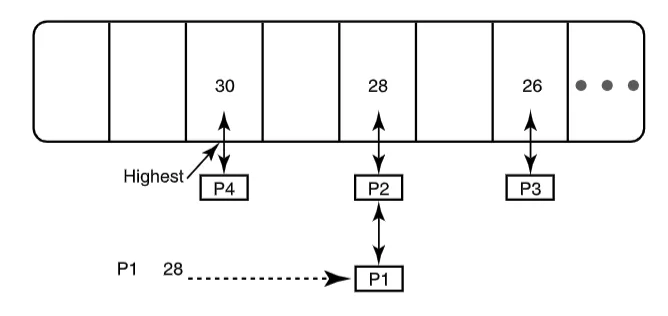
\includegraphics[width=0.8\textwidth]{../assets/ch01/ch01-1_7_端_协议处理-001.png}
\end{figure}
图9.1所示，这种分配器的工作方式是在大的内存块中进行分配。每个内存块按顺序分配，有
    一个指针Curr指向最后一次分配结束的位置。大小为B的新请求在Curr之后进行分配，然后Curr增加
    到Curr + B。这种方式速度极快，能处理可变大小的请求，并且在内存块被用完之前不会浪费任何
    内存。
其思路是，当一个内存块用完时，另一个内存块可以立即使用。当然，天下没有免费的午餐，在使用第
二个内存块时，必须在后台创建一些备用内存块。备用内存块的创建可以由软件完成，而分配操作可以
很容易地在硬件中实现。类似的想法在麻省理工学院的J机器（达利等人，1987年）中也有体现，J机器
依赖于底层的快速消息传递服务。
创建备用内存块有很多方法。当然，问题在于释放操作的顺序可能与分配操作不同，这会在内存块中产
生一组空洞，需要以某种方式进行合并。有三种合并空洞的方法。如果应用程序知道最终所有分配的缓
冲区都会被释放，那么使用更多的备用内存块可能就足以确保在任何一个内存块用完之前，有某个内存
块能被完全清理出来。然而，这是一种有风险的做法。


                                                         4
图9.1 从大内存块中顺序分配并使用备用内存块。其巧妙之处在于利用完全分配一个内存块所需的时间来
创建一个新的内存块。
其次，如果内存是通过间接寻址访问的，比如在虚拟内存中，并且缓冲区是在虚拟内存中分配的，那么
可以使用页面重映射将许多分散的物理内存页面聚集在一起，使其看起来像一个连续的虚拟内存块。最
后，还可以考虑内存压缩。在像UNIX这样的通用分配器中，内存压缩显然是不可接受的，因为可能有任
意数量的内存块指向一个内存节点。然而，在使用缓冲区或其他树状结构的网络应用中，使用简单的局
部压缩方案（西卡和瓦格赫斯，2000年），内存压缩可能是可行的。
9.1.2 共享缓冲区
如果说缓冲区分配已经够难了，那么再加上公平性约束，就更具挑战性了。假设一个实现希望在多个用
户之间公平地共享一组缓冲区，每个用户都可能希望使用所有的缓冲区。这些缓冲区应该大致平均地分
配给需要它们的活跃用户。这类似于经济学中的帕累托最优，也与第14章中研究的路由器公平排队要求
相似。因此，在随机公平排队（SFQ）算法的背景下发明了以下缓冲区窃取算法（麦肯尼，1991年）也
就不足为奇了。
 ● 缓冲区窃取：一种在用户之间大致实现帕累托最优的方法如下。当所有缓冲区都被用完，而一个新
   用户（其分配的缓冲区比当前最大分配量小）还想要一个缓冲区时，就从拥有最多缓冲区的用户那
   里窃取一个额外的缓冲区。很容易看出，即使一开始某个用户占用了所有缓冲区，当其他用户变得
   活跃时，他们也可以通过窃取获得公平的份额。
问题在于，缓冲区窃取问题的一般解决方案需要使用堆。堆的时间复杂度为O(log n)，其中n是当前有分
配的用户数量。如何才能加快速度呢？
同样，在算法学与算法的对比中，问题往往源于对规范的过度解读。如果分配量不断以任意增量变化，
并且算法总是希望找到最大的分配量，那么就需要使用对数堆实现。然而，如果我们可以放宽规范（在
实际中这似乎是合理的），假设用户每次只窃取一个缓冲区，那么分配量的变化就不是任意的，而只是
增加或减少1。这一观察结果产生了一种常数时间算法（麦肯尼算法，\begin{figure}[htbp]
\centering
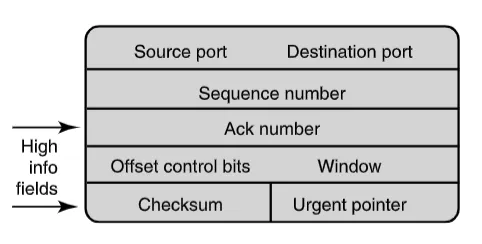
\includegraphics[width=0.8\textwidth]{../assets/ch01/ch01-1_7_端_协议处理-002.png}
\end{figure}
图9.2），该算法还假设缓冲区分配

                                                 5
量落在一个有限的集合内。对于每个分配大小i，该算法维护一个包含所有分配大小恰好为i的进程的列
表。算法还维护一个名为Highest的变量，它指向任何进程的最大分配量。
当进程P希望窃取一个缓冲区时，算法会在Highest指向的列表头部找到分配量最大的进程Q。在此过程
中，进程P获得一个缓冲区，进程Q失去一个缓冲区。记录更新如下：当进程P获得缓冲区i + 1时，P从列
表i中移除并添加到列表i + 1中，必要时更新Highest。当进程Q失去缓冲区i + 1时，Q从列表i + 1中移除
并添加到列表i中，如果Highest指向的列表变为空，则更新Highest = i。
请注意，如果P和Q的分配量变化大于1，这个算法可能会变得效率极低。例如，如果Q的分配量减少
100，并且没有其他用户具有相同的原始分配量，那么算法将需要遍历100个列表，寻找下一个可能的最
大分配量。由于分配量的最大变化量为1，所以算法只需要遍历一个列表。从算法学的角度来看，这是利
用有限全域创造特殊机会的一个例子（原则P14建议对有限全域使用桶排序和位图）。




图9.2 麦肯尼缓冲区窃取算法利用每次操作缓冲区值最多变化1这一事实，巧妙地避免了对数堆带来的开
销。
 ● 动态阈值：在共享内存交换机（第13章）中，限制任何一个流对共享缓冲区的访问也很重要。在共
   享内存交换机的背景下，乔杜里（Choudhury）和哈内（Hahne）描述了一种类似于缓冲区窃取的
   算法，他们称之为Pushout。然而，即使使用麦肯尼（1991年）的缓冲区窃取算法，Pushout在高速
   实现时可能也很困难。
相反，乔杜里和哈内（1998年）提出了一种有用的替代机制，称为动态缓冲区限制。他们观察到，为每
个流维护一个固定的阈值，要么限制过度（如果阈值太小），要么过于危险（如果阈值太大）。使用固
定的阈值与使用固定窗口大小进行流量控制没有区别。但是TCP使用动态窗口大小来适应拥塞情况。同
样，利用自由度（原则P13）并使用动态阈值是有意义的。
直观来讲，TCP窗口流量控制机制会在出现未被使用的带宽（通过数据包无丢失情况来衡量）时，增大
连接的窗口大小。同样，在共享缓冲区中适应拥塞的最简单方式，是监测剩余的空闲空间，并根据空闲
                                                          6
空间的大小按比例提高阈值。因此，用户所使用的空间被限制在不超过$cF$字节，其中$c$为常数，
$F$是当前的空闲空间量。如果将$c$选为2的幂次方，该方案仅需使用一个移位器（用于乘以$c$ ）和
一个比较器（用于与$cF$进行比较）。这甚至比缓冲区窃取算法要简单得多。
乔杜里（Choudhury）和哈内（Hahne）推荐$c$的值为1。这意味着单个用户被限制使用不超过可用带
宽的一半。这是因为当用户使用了一半带宽时，剩余的空闲空间就等于该用户的分配量，此时阈值检查
就会不通过。同样地，如果$c = 2$，任何用户被限制使用不超过可用缓冲区空间的$\frac{2}{3}$。因
此，与缓冲区窃取算法不同，这种方案总是会为新到来的用户预留一些空闲空间，用略微欠佳的内存使
用效率来换取更简单的实现方式。
现在假设有两个用户，且\(c = 1\)。有人可能会天真地认为，既然每个用户被限制使用不超过一半的资
源，那么两个活跃用户就只能使用四分之一的资源。然而，该方案的表现更好。现在每个用户可以使用
三分之一的资源，还剩下三分之一的空闲资源。接下来，如果有两个新用户到来，而老用户不释放他们
的缓冲区，那么这两个新用户最多可以获得九分之一的缓冲区空间。
因此，与缓冲区窃取算法不同，这种方案在短期内并不公平。然而，如果同一组用户存在的时间足够
长，从长期来看，这种方案应该是公平的。在前面的例子中，当分配给前两个用户的缓冲区被释放后，
应该会产生更公平的分配结果。
9.3 通用协议处理
9.1节介绍了数据包的缓冲技术，9.2节介绍了高效计算数据包校验和的技术。现在，我们可以着手实际处
理这样的数据包了。不熟悉TCP的读者可能需要先查阅第2章中的相关模型。
由于在大多数站点中，TCP流量占比达90%（布劳恩，1998年），因此以接近线速高效处理TCP数据包
至关重要。遗憾的是，乍一看，TCP代码令人望而生畏。虽然TCP发送方代码相对简单，但史蒂文斯
（1994年）指出：“TCP输入处理是我们在本文中研究的最大代码块。tcp_input函数大约有1100行代
码。处理传入的段并不复杂，只是冗长且繁琐。”
鉴于TCP看起来较为复杂，格雷格·切森（Greg Chesson）和拉里·格林（Larry Green）在1987年成立
了Protocol Engines公司，并提出了一种名为XTP的替代协议（切森，1989年）。XTP经过精心设计，
其数据包头部易于解析，处理路径也经过优化。随着XTP对TCP构成替代威胁，范·雅各布森（Van
Jacobson）在BSD UNIX中精心调整了TCP的实现，这在史蒂文斯（1994年）的著作中有详细描述。该
实现甚至能够跟上100 Mbps的链路速度。结果，尽管XTP仍在使用（切森，1989年），但TCP取得了巨
大的成功。
雅各布森优化实现的核心是一种称为头部预测的机制（雅各布森，1993年）。在处理这1100行TCP接收
处理代码时，大部分复杂性源于处理罕见情况。头部预测通过优化常见情况（原则P11），为穿越复杂的
异常情况提供了一条快速路径。
9.3.1 TCP头部预测
                                                           7
接收TCP数据包时的第一个操作是找到协议控制块（PCB），其中包含该数据包所属连接的状态（例如
接收和发送序列号）。假设连接已建立，并且大多数工作站只有少数几个并发连接，那么可以缓存这些
活动连接块。BSD UNIX代码（史蒂文斯，1994年）维护一个“滞后一个”的缓存，其中包含最后接收段
的PCB；在实际的工作站实现中，这种方法效果良好。
找到PCB后，必须处理TCP头部。帕特里奇（Partridge，1993年）提出了一种理解头部预测的有效方
式，即查看TCP头部中的字段，如\begin{figure}[htbp]
\centering
\includegraphics[width=0.8\textwidth]{../assets/ch01/ch01-1_7_端_协议处理-007.png}
\end{figure}
图9.7所示。
连接建立后，目的端口和源端口固定不变。由于IP网络会尽力按顺序发送数据包，序列号很可能是最后
接收数据包的序列号的下一个。控制位（通常称为标志位）通常为关闭状态，但确认（ack）位除外，在
发送初始数据包后，ack位始终为开启状态。最后，大多数情况下，接收方不会更改其窗口大小，紧急指
针也无关紧要。因此，信息含量较高的只有确认号和校验和字段。
基于这一观察，头部预测将常见情况确定为以下两种可能之一：接收纯确认数据包（即接收的段不包含
数据）或接收纯数据数据包（即接收的段包含的ack字段不传达新信息）。此外，数据包还应在以下精确
意义上反映正常情况：没有设置意外的TCP标志位，并且数据包中通告的流量控制窗口应与接收方先前
通告的窗口相同。用伪代码表示（简化自雅各布森，1993年）：




图9.7 TCP头部字段：最可能变化的字段是校验和和确认字段。其他字段携带的信息很少，通常可以根据
过去的值进行预测。
  1   IF (无意外标志位) AND (数据包中的窗口与之前相同)
  2      AND (数据包序列号为下一个预期值) THEN
  3           数据包仅包含头部且无数据)
           IF (
  4           执行确认处理
  5           /* 释放已确认字节，停止定时器，唤醒进程 */
  6       ELSE IF (数据包未确认任何新内容) /* 纯数据 */
  7           将数据复制到用户缓冲区，同时计算校验和；
  8           更新下一个预期序列号；
  9           如有需要，发送确认并释放缓冲区；
 10       ENDIF
 11   ELSE /* 头部预测失败 -- 采用常规处理路径 */


                                                    8
显然，这段代码比完整的TCP接收处理代码短得多。然而，利用大多数机器能够以机器字大小为单位进
行高效比较这一事实（原则P4a，利用局部性），可以使一些检查更高效。
例如，考虑图9.7控制位中的TCP标志位。共有六个标志位，每个标志位都编码为一个比特：同步
（SYN）、结束（FIN）、复位（RESET）、推送（PUSH）、紧急（URG）、确认（ACK）。在正常情
况下，除了ACK必须设置且PUSH无关紧要外，所有标志位都应清零。单独检查每个条件需要执行多条指
令来提取和比较每个比特。
相反，可以注意到标志位字段是TCP头部的第四个字，并且窗口大小包含在最后16位中。在头部预测代
码中，发送方预先计算（原则P2a）这个字的预期值，方法是填充所有预期的标志位值，并使用上次通告
的窗口大小。
TCP头部第四个字的预期值存储在连接的PCB条目中。在这种设置下，前面伪代码中的前两个检查可以
通过将传入数据包中TCP头部的第四个字与PCB中存储的预期值进行比较，一次性完成。如果一切顺利
（测试表明通常如此），则仅在连接开始时计算第四个字段的预期值。正是这个测试解释了“头部预
测”这个名称的由来：对头部的一部分进行预测，并与传入的段进行比对。
前面描述的伪代码源自雅各布森在研究内核中的实现（雅各布森，1993年），据称该实现仅用30条Sun
SPARC指令就能完成TCP接收处理！史蒂文斯（1994年）给出的BSD UNIX代码稍微复杂一些，因为它
必须处理mbufs，并且需要排除其他可能性，例如PAWS（TCP序列号回绕）测试（史蒂文斯，1994
年）。
到目前为止，我们的讨论仅限于TCP接收处理，因为它比发送TCP段更复杂。然而，发送方也存在与头
部预测类似的机制。如果各个段之间只有少数字段发生变化，发送方可以从在连接块中保留一个模板
TCP（和IP）头部中受益。发送段时，发送方只需将变化的少数字段填充到模板中。如果复制TCP头部比
逐个填充每个字段更高效，那么这种方法就更具优势。Linux内核中实现了发送数据包头部的缓存机制。
在结束这个话题之前，值得回顾注意事项Q8，并审视这种优化对系统环境的敏感程度。最初，头部预测
是针对工作站设计的。其基本假设（下一个段属于同一连接，并且序列号比最后接收的段的序列号大1）
在这种情况下效果良好。
显然，在服务器环境中，下一个段属于同一连接的假设并不成立。早在雅各布森（1993年）就已指出这
一点，他建议使用端口号的哈希值来快速定位PCB。麦肯尼（McKenney）和多夫（Dove）证实，在在
线事务处理（OLTP）环境中，使用哈希查找PCB可以将接收处理速度提高一个数量级。
先进先出（FIFO）假设更难以绕过。虽然可以采用一些巧妙的方案来处理乱序数据包的序列号，但TCP
中一些更基本的协议机制依赖于FIFO假设。例如，如果数据包经常乱序，TCP接收方会发送重复确认。
在TCP的快速重传算法（史蒂文斯，1994年）中，TCP发送方会根据三个重复确认推断数据包丢失（见
第14章）。
因此，缺乏FIFO行为会导致误重传，与头部预测失败相比，这会更严重地降低性能。然而，随着TCP接
收方逐渐支持选择性确认（弗洛伊德等人，1999年），未来或许能够快速处理乱序段。

                                                    9
9.3.2 UDP处理
回想一下，UDP是没有错误恢复、拥塞控制或连接管理功能的TCP。与TCP一样，UDP通过端口号实现
多路复用和解复用。因此，UDP使应用程序能够在无需处理TCP复杂性的情况下发送IP数据报。尽管
TCP是目前占主导地位的协议，但许多重要应用，如视频会议，都使用UDP。因此，优化UDP实现也很
重要。
由于UDP是无状态的，头部预测并不适用：无法存储过去的头部信息来预测未来的头部。然而，UDP与
TCP有两个可能耗时的相同任务：解复用至正确的PCB以及计算校验和，这两个任务都可以从类似TCP
的优化中受益（帕特里奇和平克，1993年）。
UDP中PCB条目的缓存比TCP中更复杂。这是因为在查找PCB时，可能需要使用通配符条目来匹配远程
（称为外部）IP地址和端口。例如，可能存在PCB 1，它指定本地端口L，而其他所有字段均为通配符；
还可能存在PCB 2，它指定本地端口L和远程IP地址X。如果缓存了PCB 1，而到达的数据包目的地是
PCB 2，那么缓存可能会导致数据包被错误地解复用至PCB 1。因此，一般情况下无法缓存通配符条目；
出于类似原因，在路由查找（第11章）中也不能缓存地址前缀。
帕特里奇和平克（1993年）提出了一种简单策略来解决这个问题。像PCB 1这样可能“隐藏”或匹配其他
PCB条目的条目，绝不允许被缓存。在这个限制条件下，帕特里奇和平克（1993年）的UDP实现会缓存
最后接收数据包的PCB和最后发送数据包的PCB。第一个缓存用于处理连续接收的数据包，而第二个缓
存用于处理常见的情况，即接收到对最后发送数据包的响应。尽管存在缓存限制，但在帕特里奇和平克
（1993年）的测量中，这两个缓存的命中率仍达到87%。
最后，帕特里奇和平克（1993年）还为UDP实现了与TCP类似的复制和校验和循环。在BSD实现中，
UDP的sosend函数被视为通过已连接套接字发送数据的特殊情况。相反，帕特里奇和平克提出了一种高
效的专用例程（原则P6），该例程首先计算头部校验和，然后在将数据字节复制到网络缓冲区的同时更
新校验和。（其中一些想法使Cray机器在20世纪90年代初能够对校验和循环进行向量化处理。）在接收
处理中采用类似的优化措施后，帕特里奇和平克报告称，对于受内存访问时间而非处理能力限制的
CPU，校验和计算的成本基本为零。
9.4 重组
TCP的头部预测以及帕特里奇和平克（1993年）对UDP的优化，都假设接收的数据流无需进行特殊计
算。例如，假设TCP段不包含窗口大小变化或不需要关注的标志位设置。此外，到目前为止，还有一个
未明确说明的假设，即IP数据包无需重组。
简而言之，最初的IP路由协议通过允许路由器将IP数据包分片，来处理具有不同最大数据包大小或最大传
输单元（MTU）的各种链路。每个分片由数据包ID、在原始数据包中的起始字节偏移量和分片长度标
识。最后一个分片会设置一个比特位，以表明它是最后一个分片。需要注意的是，中间路由器可能会导
致一个分片进一步被分割成多个更小的分片。IP路由还可能导致分片重复、丢失和乱序接收。

                                                10
在接收方，“破碎的蛋”（即原始数据包）可以按以下方式重新组装。第一个到达接收方的分片会建立以
相应数据包ID为索引的状态。后续的分片会被引导至相同的状态（例如，基于数据包ID的分片链表）。
如果接收到最后一个分片，并且其余分片覆盖了原始数据包长度中的所有字节（由每个分片的偏移量指
示），接收方就可以判断数据包已完整。如果在指定时间内数据包未完成重组，则该状态将超时。
虽然分片使IP能够处理不同MTU大小的链路，但它存在以下缺点（肯特和莫古尔，1987年）。首先，路
由器对数据包进行分片的成本较高，因为这需要为每个分片添加新的IP头部，从而增加了处理和内存带
宽需求。其次，在终端节点进行重组的成本也较高，因为确定一个完整的数据包是否已组装完成，可能
需要对接收的分片进行排序。第三，一个分片的丢失会导致整个数据包丢失；因此，当一个分片丢失
时，传输其余的分片就是在浪费资源。
当前的互联网策略（肯特和莫古尔，1987年）是将分片计算在空间上（原则P3c）从路由器和接收方转
移到发送方。所谓的路径MTU方案的核心思想是，发送方有责任计算出一个足够小的数据包大小，以确
保数据包能够通过从发送方到接收方路径上的所有链路。现在，路由器可以拒绝分片数据包，并向接收
方发送控制消息。发送方使用常见数据包大小列表（原则P11，优化常见情况），在收到拒绝消息时，从
该列表中选择较小的数据包大小。
路径MTU方案通过将问题转移到系统的其他部分，很好地展示了算法的实际应用。然而，有一种误解认
为路径MTU已完全消除了互联网中的分片现象。事实并非如此。几乎所有核心路由器都支持硬件分片，
并且在路径MTU协议部署多年后，在互联网骨干链路上仍观察到大量分片流量（香农等人，2001年）。
需要注意的是，路径MTU协议要求发送方在PCB中保存当前最佳数据包大小的状态信息。如果发送方使
用TCP，这种方式效果良好，但如果发送方使用无状态的UDP，情况就不同了。在UDP的情况下，只有
当UDP之上的应用程序保存必要的状态并实现路径MTU（除非路径MTU像在IBM AIX系统中那样存储为
路由表条目）时，才能实现路径MTU。这更难部署，因为与仅更改TCP相比，更改众多应用程序更加困
难。因此，在撰写本文时，诸如NFS之类的共享文件系统协议、IP-in-IP封装协议以及许多媒体播放器和
游戏协议都基于UDP运行，并且不支持路径MTU。最后，许多攻击者会将攻击负载分散在多个分片中，
从而危及安全性。因此，入侵检测设备通常必须重组IP分片，以检查重组数据中是否存在可疑字符串。
因此，研究快速重组算法很有必要，因为像NFS这样的常见程序不支持路径MTU协议，并且实时入侵检
测系统必须以线速重组数据包，以检测隐藏在分片中的攻击。下一节将介绍接收方的快速重组实现。
9.4.1高效重组
\begin{figure}[htbp]
\centering
\includegraphics[width=0.8\textwidth]{../assets/ch01/ch01-1_7_端_协议处理-008.png}
\end{figure}
图9.8展示了一种简单的数据结构，类似于BSD UNIX中用于重组数据包的数据结构。假设有三个ID为
1080的数据包分片已经到达。这些分片按照起始偏移量在列表中进行排序。注意，这里存在字节重叠的
情况，因为第一个分片包含字节1-10，而第二个分片包含字节2-21。



                                                  11
图9.8 一种用于重组的数据结构是一个由数据包ID索引、按起始字节偏移量（第一个字段）排序的分片链
表。第二个字段是结束偏移量。因此，起始偏移量为25的分片会插入到列表中第二个元素之后。
因此，如果一个ID为1080、偏移量为25-30的新分片到达，实现过程通常会从列表头部开始遍历，以找
到正确的插入位置。正确的位置在起始偏移量2和40之间，也就是在第二个列表项之后。
每次将一个分片放入列表时，在遍历列表的过程中，实现可以检查到该分片为止是否已经接收到了所有
需要的字节。如果是，它会继续检查列表末尾，看是否接收到了所有字节，并且最后一个分片的最后分
片位是否被设置。如果满足这些条件，就说明所有需要的分片都已到达；然后实现会再次遍历列表，将
每个分片的数据按指定偏移量复制到另一个缓冲区中，有可能避免复制重叠部分。
最终的实现相当复杂且速度较慢，通常还需要额外的复制操作。需要注意的是，要插入一个分片，必须
先找到数据包ID对应的列表，然后在列表中进行搜索。这需要两次线性搜索。IP重组本质上就这么困难
吗？
奇怪的是，存在一种反例重组协议，它已在硬件中实现了千兆速度：ATM AAL - 5信元重组协议（帕特
里奇，1993年），该协议主要描述了如何将IP数据包分割成53字节的ATM信元，并在接收端将信元重组
为数据包。AAL - 5重组算法在硬件中易于实现的原因，并非是固定长度的信元（该实现可以推广到可变
长度的信元），而是信元只能按先进先出（FIFO）顺序到达。
如果信元只能按FIFO顺序到达，那么很容易将每个后续信元粘贴到前一个信元之后的缓冲区中。当携带
最后信元位的最后一个信元到达时（就像在IP中一样），会检查数据包的CRC。如果CRC计算正确，数
据包就成功重组。需要注意的是，ATM不需要任何偏移量字段，因为数据包在ATM虚拟电路中是按顺序
到达的。
与ATM信元不同，IP数据报理论上可以以任何顺序到达，因为IP采用数据报（邮政）模型，而非虚拟电
路（电话）模型。然而，我们刚刚看到，头部预测，实际上还有快速重传算法，都关键依赖于在预期情
况下IP段按顺序到达这一事实（原则P11，优化预期情况）。结合这一观察和AAL - 5的实现可知，通过
针对分片按FIFO顺序到达的情况进行优化，甚至在硬件中也可以获得一种高效的重组算法，如\begin{figure}[htbp]
\centering
\includegraphics[width=0.8\textwidth]{../assets/ch01/ch01-1_7_端_协议处理-009.png}
\end{figure}
图9.9所
示。




                                                 12
图9.9 这种实现与图9.8类似，只是针对分片不重叠且按顺序到达的情况进行了优化。
图9.9与图9.8一样维护了一个已排序的列表，同时还保留了一个指向列表末尾的指针。针对分片按顺序
且不重叠到达的情况进行优化后，当包含字节22-30的分片到达时，实现会将最后接收分片的结束字节
数（存储在寄存器中，等于21）与新分片的起始偏移量进行比较。由于22等于21 + 1，一切正常。新的
结束字节更新为新分片的结束字节（30），并且在将新到达的分片链接到列表末尾后，指针也更新为指
向该分片。最后，如果新到达的分片是最后一个分片，重组就完成了。
与图9.8中的实现相比，检查重组是否完成以及确定分片插入位置的操作所花费的时间是常数级的，而非
线性级的。同样，可以缓存预期的数据包ID（就像在TCP或UDP的PCB查找实现中那样），以避免在搜
索分片列表时遍历列表。最后，使用pbufs等数据结构而非mbufs，甚至可以通过将接收到的分片直接按
适当偏移量复制到缓冲区中，避免额外的复制操作。
如果预期情况未发生，实现可以恢复到标准的BSD处理方式。例如，钱德兰梅农（Chandranmenon）和
瓦格赫斯（Varghese）在1998年描述了这种预期情况优化方法，代码会维护两个列表，当预期情况未发
生时，会直接重用现有的BSD代码（这些代码很难编写正确！）。钱德兰梅农和瓦格赫斯在1998年报告
称，预期情况的处理需要38条SPARC指令，这与雅各布森对TCP处理的估计相当。
与头部预测一样，值得应用注意事项Q8，审视这种实现的优化对假设条件的敏感程度。实际上，结果相
当不理想。因为测量表明，包括Linux在内的许多最新实现中，发送方会以相反的顺序发送分片！因此，
9%的情况下分片会以相反的顺序到达（香农等人，2001年）。
这种看似奇怪的行为是有原因的，因为只有最后一个分片携带整个数据包的长度；假设分片按FIFO顺序
到达，发送方先发送最后一个分片，就能让接收方在收到第一个分片后知道要分配多大长度的缓冲区。
需要注意的是，FIFO假设仍然成立。然而，图9.9存在一个隐藏但微妙的额外假设：分片将按偏移量顺序
发送。在继续阅读之前，请思考如何修改图9.9的实现来处理这种情况。
当然，解决方案是使用第一个分片来决定针对两种预期情况中的哪一种进行优化。如果第一个分片是起
始分片（偏移量为0），那么实现会采用图9.9中描述的模式。如果第一个分片是最后一个分片（最后一
位被设置），实现会切换到不同的状态，在这种状态下它预期分片会以相反的顺序到达。这与图9.9正好
相反，在这种情况下，下一个分片的最后字节数应该比前一个分片的起始偏移量小1（而不是大1）。同
样，下一个分片预期会粘贴到列表的开头，而不是末尾。

                                                   13
9.5结论
本章介绍了高效的缓冲区分配、CRC和校验和计算、TCP等协议处理，以及最后的数据包重组技术。
对于缓冲区分配，诸如使用分离池和批量分配等技术有望实现快速分配，但也存在潜在的权衡：分离池
技术缺乏存储效率，而批量分配技术则面临合并不连续空洞的困难。缓冲区共享对于高效利用内存非常
重要，可以通过从大用户那里高效窃取缓冲区或使用动态阈值来实现。
对于CRC计算，高效的多位余数计算避免了逐位计算CRC的明显浪费（原则P1），即使是使用线性反馈
移位寄存器（LFSR）实现也是如此。对于校验和计算，主要技巧是根据底层机器架构进行计算，使用大
的字长、延迟进位检查，甚至并行计算。对TCP、UDP和数据包重组的优化都基于对简单预期情况（例
如FIFO接收、无错误）的优化，这些优化能够避开协议必须检查但很少出现的大量特殊情况。表9.1总结
了本章使用的技术以及涉及的主要原则。
除了具体的技术，还可以从中获得一些一般性的经验教训。第一，在考虑缓冲区窃取算法时，人们很容
易认为找到拥有最大缓冲区分配的用户需要使用堆，这需要对数时间复杂度。然而，就像第7章中的定时
轮一样，麦肯尼算法利用了缓冲区大小仅增加或减少1的特殊情况。
一般的经验是，对于算法学来说，特殊情况很重要。理论家们深知这一点；例如，寻找哈密顿回路的一
般问题（科曼等人，1990年）对于一般图来说很难，但如果图是一个环，问题就很简单。实际上，算法
学的实践者应该寻找机会改变系统，以允许出现能够使用高效算法的特殊情况。
第二，动态阈值方案表明优化自由度（原则P13）非常重要，尤其是在考虑参数的动态而非静态值时。这
是许多协议中非常常见的演进路径：例如，以太网中的冲突避免协议从使用固定的退避时间演进到使用
动态退避时间；传输协议从使用固定窗口大小演进到使用动态窗口大小以适应拥塞；最后，本章的动态
阈值方案展示了允许动态缓冲区阈值的优势。
第三，对缓冲区共享技术的讨论说明了算法学的作用，至少在抽象常见网络任务以及理解这些任务的多
种解决方案方面是有用的。例如，在撰写本章时发现，缓冲区共享也是许多基于信用的协议（如奥兹韦
伦等人，1994年，见第15章中的协议）的一部分，只是在这种情况下，发送方是在远程接收方分配缓冲
区空间。分离出抽象问题很有帮助，因为这表明，例如，乔杜里和哈内的动态阈值方案比奥兹韦伦等人
（1994年）的技术能够提供更精细的缓冲区共享。
最后，从头部预测和快速重组中得到的最后一个经验教训是，为实现更快速度而设计新协议的尝试，往
往可以被更简单的实现所取代。特别是，如果在预期情况下能够巧妙处理协议的复杂性，那么声称某个
协议 “复杂” 往往就无关紧要了。
再举一个例子，一种传输协议（萨布纳尼和内特拉瓦利，1989年）被设计用于为使用大窗口且能处理乱
序交付的协议提供高效的序列号处理。该协议为此目的在协议中嵌入了连续序列号块等概念。专利（托
马斯等人，1992年）中描述的简单实现技巧，通过使用大的字来有效地表示序列号块，而无需重新设计
协议，就可以达到类似的效果。

                                                14
因此，历史告诉我们，对于为提高效率（而非增加更多功能）而重新设计协议的尝试，应该持一定的怀
疑态度。




                                            15
